\clearpage
\section{إجراءات التشغيل القياسية}
\label{sec:builder-feature-sops}

تفتح هذه الصفحة استوديو أتمتة مضمّناً يبني مسارات تربط كيان بحسابات وخدمات أخرى، وتبدأ بحدث في كيان مثل إنشاء سجل أو إرسال نموذج. وتعمل كل أتمتة فيه من خلال اتصال بحساب كيان تختاره أولاً. أما مسارات الاعتماد والمهام داخل المؤسسة فالأنسب لها «الإجراءات الداخلية».

\textbf{المسار ومن يستخدمه:} «ادوات البناء» ← «الأساسية» ← «إجراءات التشغيل القياسية». يستخدمها من يملك صلاحية النماذج ويحتاج إلى ربط كيان بأنظمة أخرى.

\begin{rcnote}[مثال: شركة الأفق]
تريد الأفق أن تصل رسالة إلى جدول متابعة خارجي كلما أُنشئ طلب زيارة. لذلك يبني مسؤول النظام أتمتة تبدأ عند إنشاء سجل جديد في «طلبات الزيارة»، ثم تتحقق من الفرع قبل أن ترسل البيانات.
\end{rcnote}

\begin{table}[H]
\centering
\caption{أجزاء الأتمتة}
\label{tab:builder-sops-parts}
\begin{tabularx}{\linewidth}{R{3.6cm} Y}
\rcHeaderRow
\thh{الجزء} & \thh{المعنى}\\
الاتصال & حساب كيان الذي تعمل الأتمتة باسمه، ويُختار أولاً. اجعله بأقل صلاحيات تكفي العمل.\\
المشغّل & الحدث الذي يبدأ الأتمتة، مثل إنشاء سجل أو تحديثه أو إجراء على نموذج أو مهمة.\\
الشرط & يتحقق من البيانات قبل أي كتابة، حتى لا تعمل الأتمتة على سجلات لا تخصها.\\
الإجراءات & ما تفعله الأتمتة: إنشاء سجل أو تحديثه أو البحث عنه، وإنشاء مهام، وإرسال إشعار، وغيرها.\\
\end{tabularx}
\end{table}

\begin{figure}[H]
\centering
\begin{tikzpicture}[node distance=0.5cm]
\node[stepBox] (a) {\RL{اختيار الاتصال}};
\node[stepBox,below=of a] (b) {\RL{المشغّل}};
\node[stepBox,below=of b] (c) {\RL{شرط قبل الكتابة}};
\node[stepBox,below=of c] (d) {\RL{إجراء واحد في كل مرة}};
\draw[flowsTo] (a) -- (b);
\draw[flowsTo] (b) -- (c);
\draw[flowsTo] (c) -- (d);
\end{tikzpicture}
\rclegend
\caption{ترتيب بناء الأتمتة}
\label{fig:builder-sops-flow}
\shotnote{يضع المخطط الشرط قبل الإجراء، لأن الأتمتة التي تكتب دون تحقق قد تغيّر سجلات كثيرة في لحظة. وتُختبر الأجزاء واحداً واحداً: المشغّل وحده، ثم الشرط في الحالتين، ثم كل إجراء على حدة.}
\end{figure}

\subsection{خطوات العمل والتحقق}
\begin{enumerate}
\item افتح «إجراءات التشغيل القياسية» وأنشئ مساراً جديداً، ثم اختر اتصال كيان.
\item اختر المشغّل، واختبره ببيانات عينة.
\item أضف شرطاً يتحقق من البيانات، ثم أضف الإجراءات واحداً بعد الآخر واختبر كلاً منها.
\item فعّل الأتمتة بعد نجاح الاختبار، ثم راجع أول تشغيل فعلي.
\end{enumerate}

\textbf{تحقق ومعالجة المشكلة:} يجب أن يظهر التشغيل في سجل الأتمتة بالنتيجة المتوقعة. فإذا ظهرت الصفحة فارغة أو برسالة خطأ، فقد تكون خدمة الأتمتة غير متاحة في بيئة مؤسستك؛ وفي بيئة الاختبار \en{test2} ظهرت الصفحة فارغة عند التحقق. وإذا فشل إجراء، فراجع صلاحيات الاتصال أولاً.

\clearpage
\section{البوتات}
\label{sec:builder-feature-bots}

البوت مساعد له اسم وصورة، يضيفه الأعضاء إلى الدردشة أو البريد أو التقويم. وتحدد في هذه الصفحة أين يمكن إضافته، وهل يُضاف تلقائياً، وكيف يصل إلى البريد. أما ما يفعله البوت عندما يُراسَل أو يُذكر فيُبنى في «الإجراءات الداخلية» بمشغّلات مثل «عند رسالة مباشرة إلى الروبوت» و«عند الإشارة».

\textbf{المسار ومن يستخدمه:} «ادوات البناء» ← «الأساسية» ← «البوتات». يستخدمها من يملك صلاحية البوتات.

\begin{rcnote}[مثال: شركة الأفق]
ينشئ مسؤول النظام بوت «مساعد الزيارات»، ويجعله قابلاً للإضافة إلى الدردشات المباشرة. فإذا راسله عمر حداد، بدأ إجراء داخلي يرد عليه بحالة طلب زيارته. ويبدأ البوت من ①.
\end{rcnote}

\begin{figure}[H]
\centering
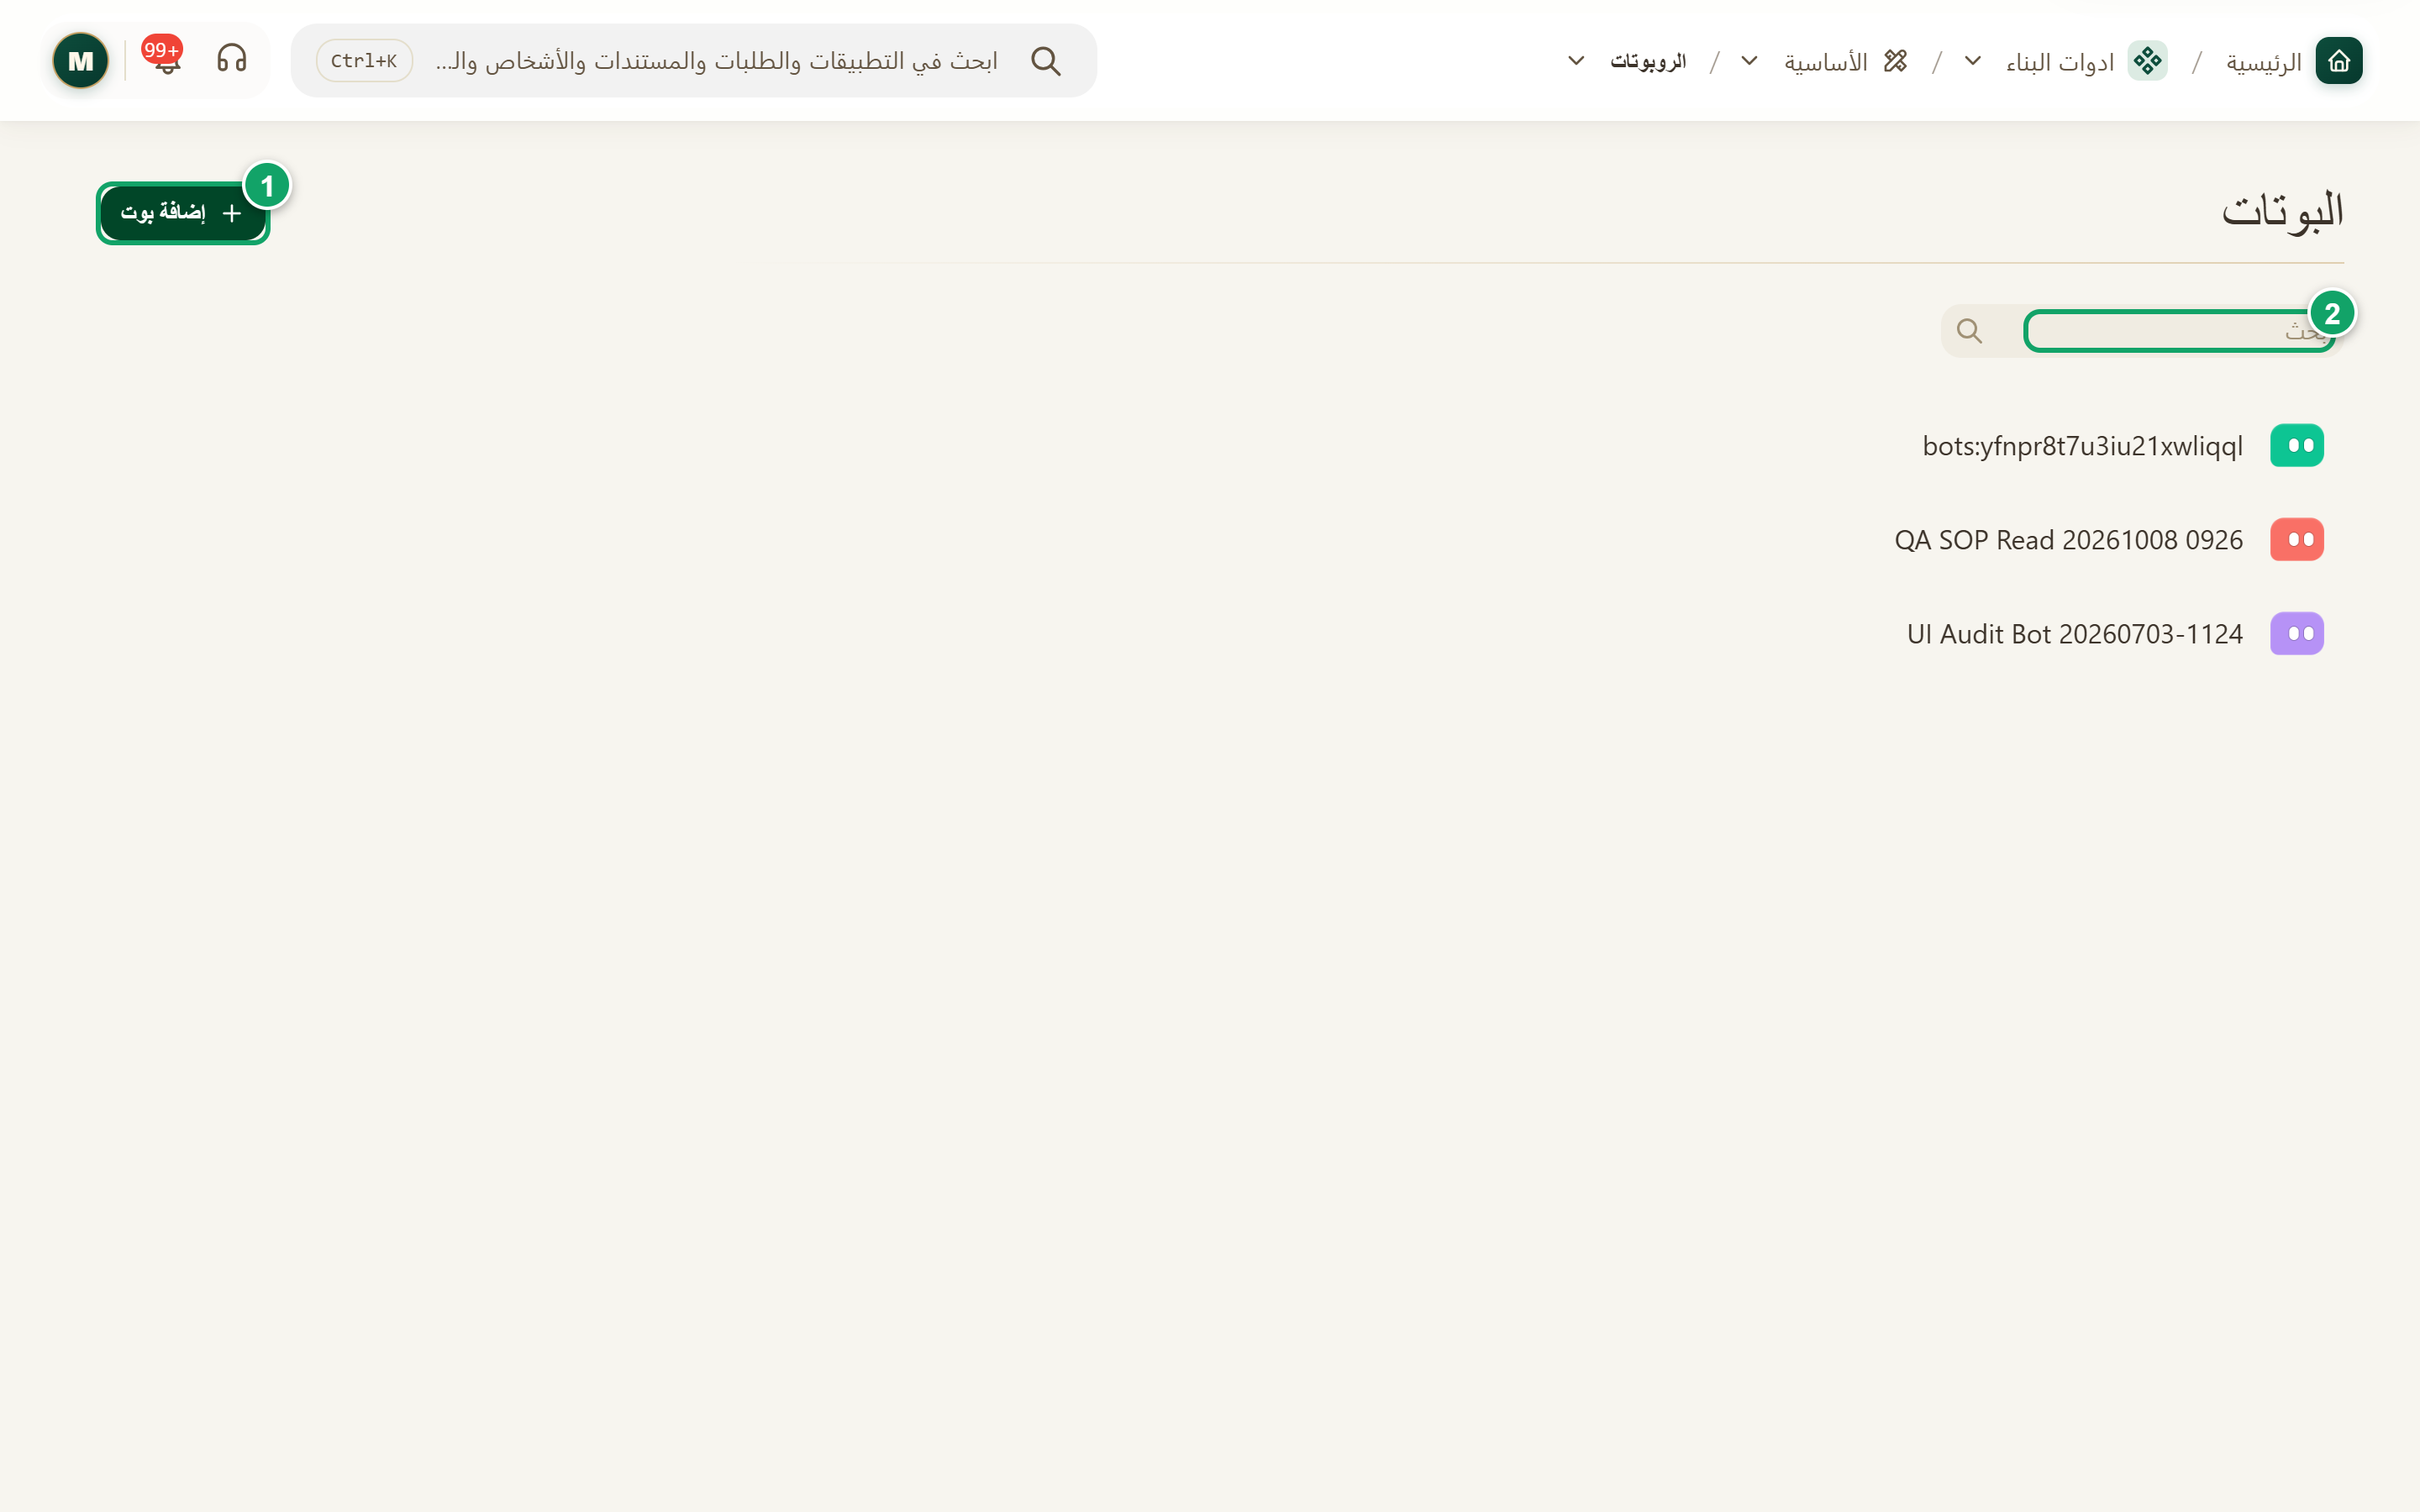
\includegraphics[width=0.95\linewidth,height=0.72\textheight,keepaspectratio]{figures/screens/ch06-bots-ar.png}
\caption{صفحة «البوتات»}
\label{fig:builder-bots-screen}
\shotnote{تعرض الصفحة البوتات المعرّفة في المؤسسة، وهي هنا بوتات اختبار. ① «إضافة بوت»: يطلب الاسم فقط. ② البحث: يجد البوت بالاسم.}
\end{figure}


\begin{table}[H]
\centering
\caption{إعدادات البوت}
\label{tab:builder-bots-data}
\begin{tabularx}{\linewidth}{R{3.6cm} Y}
\rcHeaderRow
\thh{القسم} & \thh{ماذا تحدد؟}\\
إضافة بوت & يطلب الاسم فقط، وتُختار صورته تلقائياً.\\
الدردشة & هل يُضاف إلى الدردشات المباشرة أو القنوات، وهل يمكن مراسلته أو ذكره.\\
البريد الإلكتروني & هل يُثبّت في البريد، وهل يمكن إضافته في نسخة، وإضافة جهات اتصال داخلية أو خارجية.\\
التقويم & هل يمكن تثبيته في التقويم.\\
التثبيت الافتراضي & هل يُضاف تلقائياً إلى الدردشة أو البريد أو التقويم، وحدود وصوله الافتراضية إلى البريد.\\
\end{tabularx}
\end{table}

\begin{figure}[H]
\centering
\begin{tikzpicture}[node distance=0.5cm]
\node[entity] (bot) {\RL{البوت}};
\node[entityOpt,below right=0.7cm and 0.3cm of bot] (where) {\RL{أين يُضاف}};
\node[entityOpt,below left=0.7cm and 0.3cm of bot] (sop) {\RL{إجراء داخلي يرد}};
\draw[dependsOnOpt] (bot.south) -- ++(0,-0.3) -| (where.north);
\draw[dependsOnOpt] (bot.south) -- ++(0,-0.3) -| (sop.north);
\end{tikzpicture}
\rclegend
\caption{هوية البوت وعمله}
\label{fig:builder-bots-model}
\shotnote{يفصل الشكل بين أمرين: هذه الصفحة تحدد هوية البوت وأماكن إضافته، أما ردوده فيبنيها إجراء داخلي يبدأ عندما يُراسَل البوت أو يُذكر. لذلك لا يفعل البوت شيئاً وحده حتى تربطه بإجراء منشور.}
\end{figure}

\subsection{خطوات العمل والتحقق}
\begin{enumerate}
\item افتح «البوتات» واضغط «إضافة بوت»، ثم اكتب الاسم واضغط «إنشاء».
\item افتح البوت، وفعّل أماكن إضافته في الدردشة والبريد والتقويم، ثم اضغط «حفظ».
\item ابنِ في «الإجراءات الداخلية» إجراءً يبدأ «عند رسالة مباشرة إلى الروبوت» وانشره.
\end{enumerate}

\textbf{تحقق ومعالجة المشكلة:} أضف البوت إلى دردشة تجريبية وأرسل إليه رسالة، فيجب أن يبدأ الإجراء ويظهر في «عمليات التشغيل». فإذا لم تظهر خيارات الإضافة للأعضاء، فراجع إعدادات الدردشة والحفظ؛ وإذا لم يرد البوت، فتأكد من أن الإجراء منشور وغير متوقف.
